
\section{Modelo Identificado}
\begin{figure}[H]
  \centering
  \includegraphics[width=0.5\textwidth]{results/all/states.pdf}
  \caption{Number of states of identified model for different values of $k$.}
    \label{fig:statesIdentOriginal}
\end{figure}
\begin{figure}[H]
  \centering
  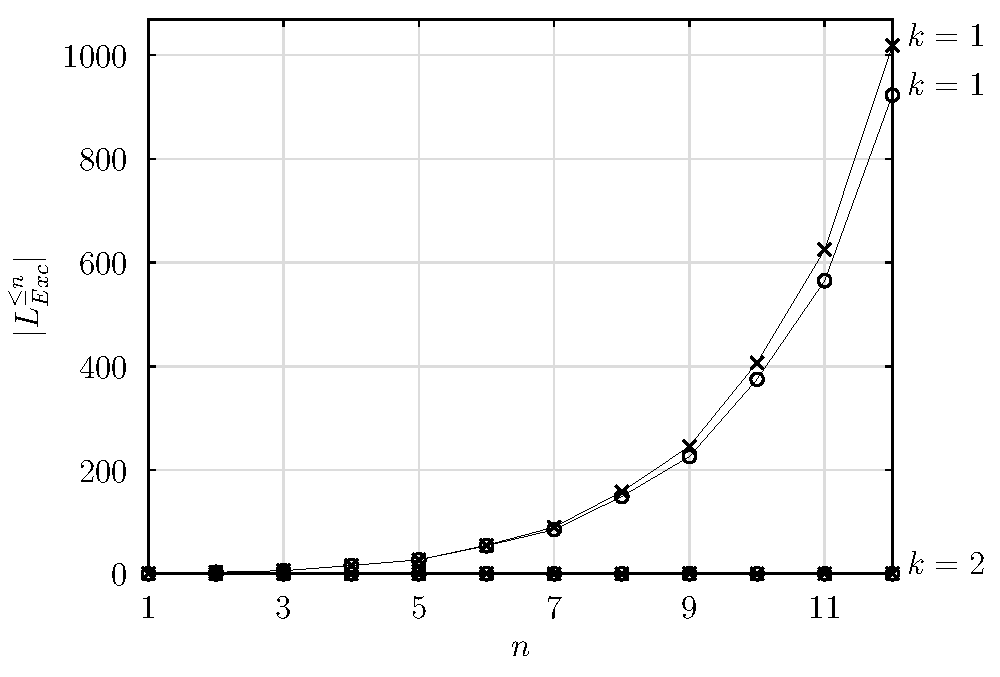
\includegraphics[width=0.5\textwidth]{results/all/exceedingLanguage-daoct-ndaao_k1-2_n12.pdf}
  \caption[Comparison between the cardinality of the exceeding language generated by the DAOCT and
NDAAO.]{Comparison between the cardinality of the exceeding language generated by the DAOCT (o) and
NDAAO ($\times$) models, for $k=1$ and $k=2$.}
    \label{fig:daoctNdaaoOriginal}
\end{figure}
\begin{figure}[H]
  \centering
  \includegraphics[width=0.5\textwidth]{results/all/best/states.pdf}
  \caption{Number of states of identified model for different values of $k$.}
    \label{fig:statesIdentBest}
\end{figure}

\begin{figure}[H]
  % \centering
  \begin{subfigure}[H]{0.5\textwidth}
    \centering
    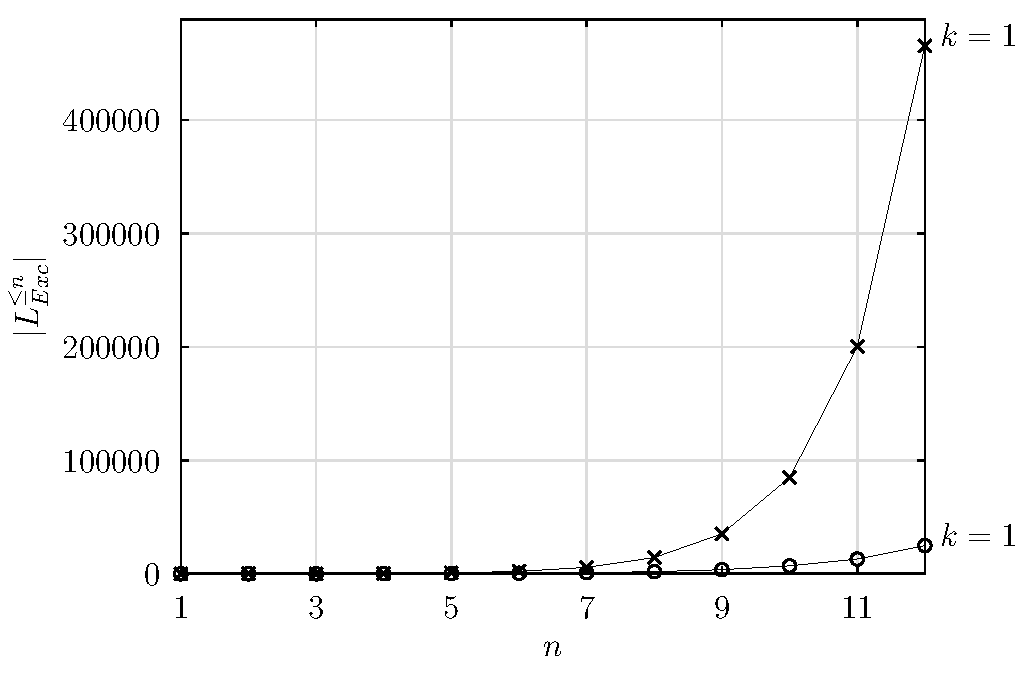
\includegraphics[width=\textwidth]{results/all/best/exceedingLanguage-daoct-ndaao_k1_n12.pdf}
    \caption{$k=1$}
    \label{fig:daoctNdaaoBestkone}
  \end{subfigure}
  ~
  \begin{subfigure}[h]{0.5\textwidth}
    \centering
    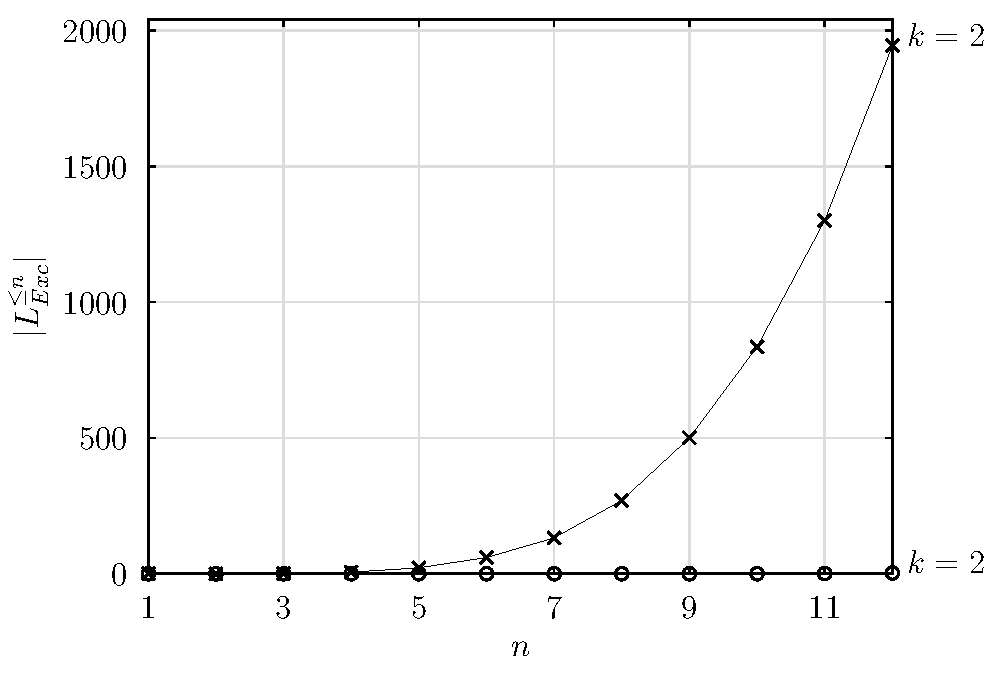
\includegraphics[width=\textwidth]{results/all/best/exceedingLanguage-daoct-ndaao_k2_n12.pdf}
    \caption{$k=2$}
    \label{fig:daoctNdaaoBestktwo}
  \end{subfigure}
  % \begin{center}
  \begin{subfigure}[h]{0.5\textwidth}
    \centering
    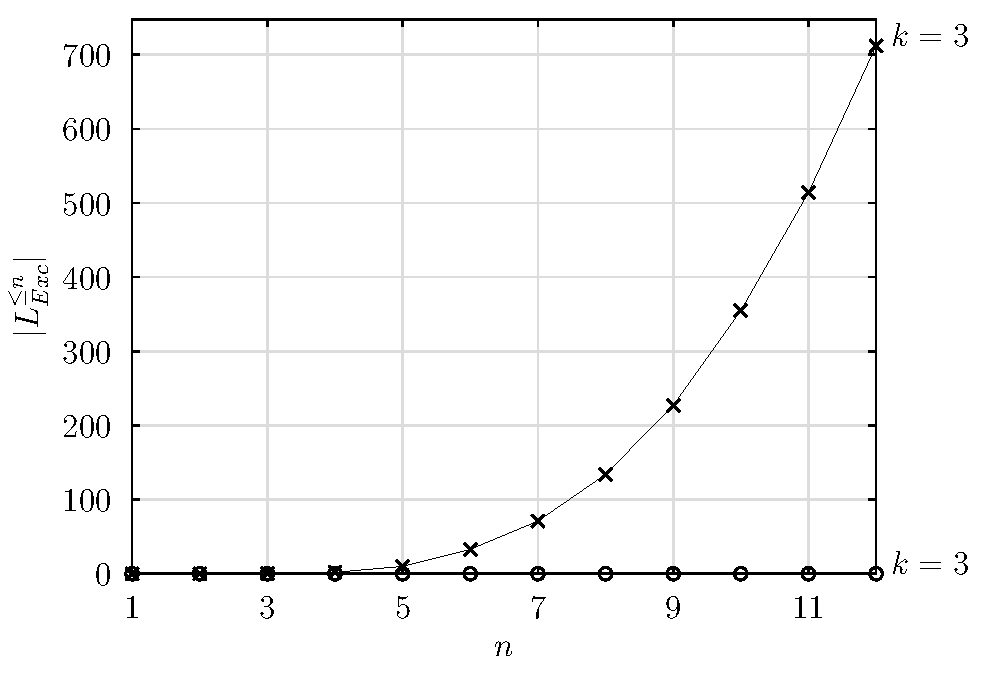
\includegraphics[width=\textwidth]{results/all/best/exceedingLanguage-daoct-ndaao_k3_n12.pdf}
    \caption{$k=3$}
    \label{fig:daoctNdaaoBestkthree}
  \end{subfigure}
  \begin{subfigure}[h]{0.5\textwidth}
    \centering
    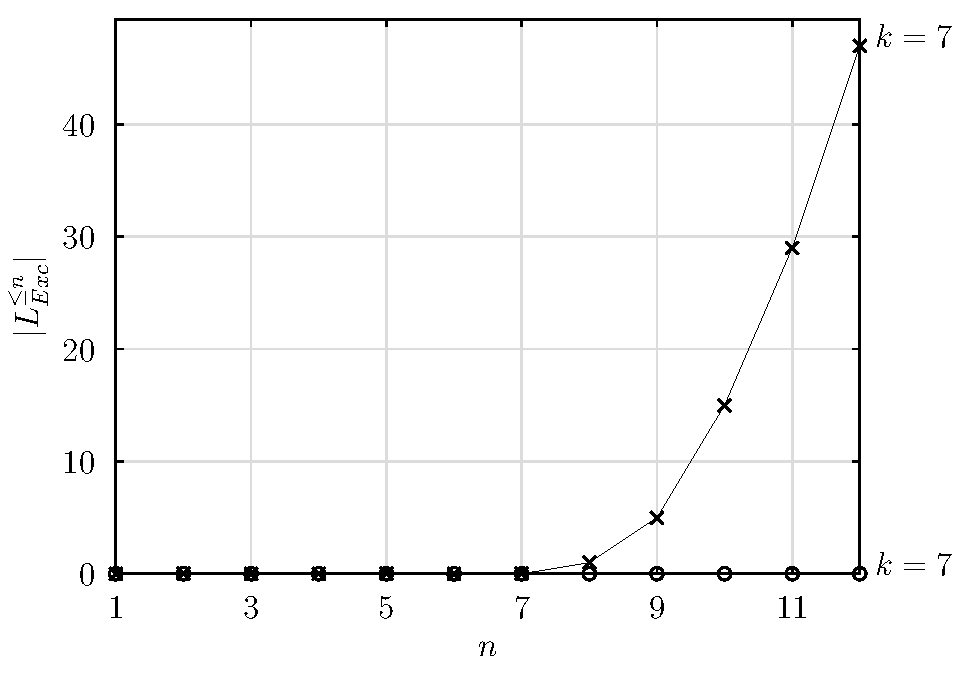
\includegraphics[width=\textwidth]{results/all/best/exceedingLanguage-daoct-ndaao_k7_n12.pdf}
    \caption{$k=7$}
    \label{fig:daoctNdaaoBestkseven}
  \end{subfigure}
    % \end{center}
  \caption[Comparison between the cardinality of the exceeding language generated by the DAOCT and
NDAAO.]{Comparison between the cardinality of the exceeding language generated by the DAOCT (o) and
NDAAO ($\times$) models.}
\end{figure}
\begin{figure}[H]
  \centering
  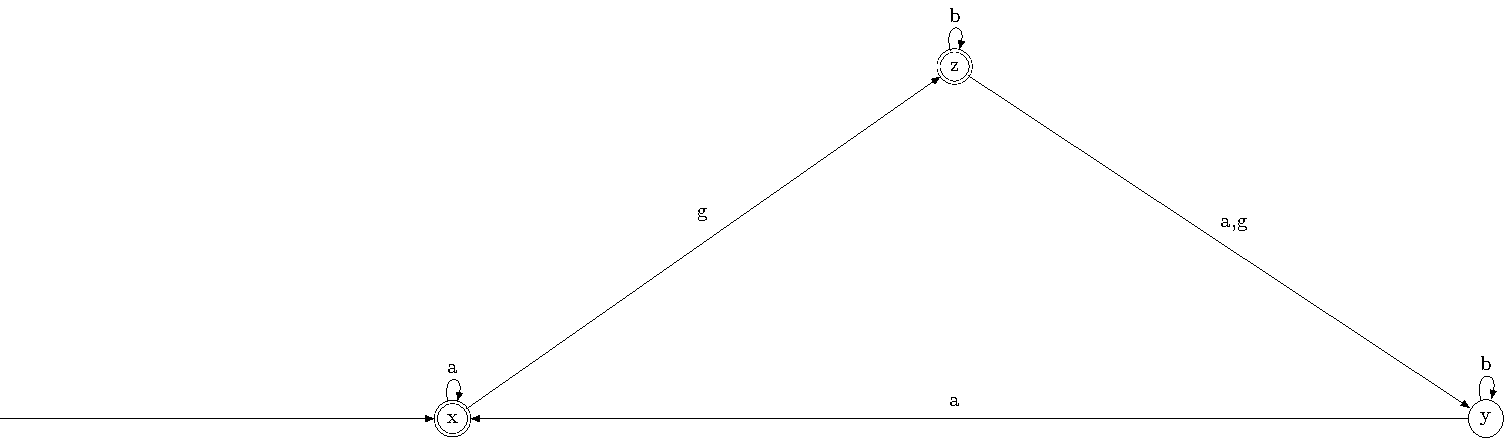
\includegraphics{results/example/example}
  \caption{Scheme of the example.}
    \label{fig:schemeExConveyor}
\end{figure}
\begin{align}
  \label{motif}
\colvec{0\\0\\0}\colvec{1\\0\\0}\colvec{0\\0\\0}\colvec{0\\1\\0}\colvec{0\\0\\0}\colvec{0\\0\\1}
\end{align}
\begin{figure}[H]
  \centering
 \includegraphics{results/example/examplek1NoArrows}
  \caption{Identified model using $\colvec{0&0&0}^T$ as initial state, $k=1$.}
    \label{fig:exampleCol000k1}
\end{figure}
  \begin{align}
\label{motifMod}
\colvec{1\\0\\0}\colvec{0\\0\\0}\colvec{0\\1\\0}\colvec{0\\0\\0}\colvec{0\\0\\1}\colvec{0\\0\\0}
\end{align}
\begin{figure}[H]
  \centering
  \includegraphics{results/example/example1k1NoArrows}
  \caption{Identified model using $\colvec{1&0&0}^T$ as initial state, $k=1$.}
    \label{fig:exampleCol100k1}
\end{figure}
\begin{figure}[H]
  \centering
  \includegraphics[width=\textwidth]{results/example/example1k2NoArrows}
  \caption{Identified model using $\colvec{1&0&0}^T$ as initial state, $k=2$.}
    \label{fig:exampleCol100k2}
  \end{figure}
\begin{align}